\documentclass[../1.tex]{subfiles}

\begin{document}

    An important field in algebraic topology is homology theory. We shall discuss homology theory to the extent
    that allows us to define the laplacian operator on simplicial complexes, for further readings see \cite{hatcher}.
    \begin{defn}
        An \ii{oriented} simplicial complex $\mc{A}$ is a simplicial complex and a partial order on $Vert(\mc{A})$ whose
        restriction to the vertices of any simplex in $\mc{A}$ is a linear order.
    \end{defn}

    \begin{defn}
        Let $\mc{A}$ be an oriented simplicial complex, on $\mc{A}$ we define a formal sum in order
        to obtain a vector space on the real numbers, that is
        \[ C_p(\mc{A}) := \{ \sum_i \lambda_i \sigma_i^p \quad \lambda_i \in \R \},\]
        where $\sigma_i^p$ are oriented p-simplexes of $\mc{A}$.\\
        All $\sigma_i^p = [v_0,\dots,v_p]$ can have two possible orientations that satisfy
        $ [v_0,\dots,v_p] = sgn (\pi)[v_{\pi 0},\dots,v_{\pi p}]$,
        where $\pi$ is a permutation of $\{0,\dots,p\}$.        
    \end{defn}

    \begin{defn}
        We define the linear operator $\del_{p+1} : C_{p+1} \to C_p$ by setting
        \[ \del_{p+1}([v_0,\dots,v_p]) = \sum_{i=0}^p (-1)^i[v_0,\dots,\hat{v_i},\dots,v_p] \]
        (where $\hat{v_i}$ means delete the vertex $v_i$) and extending by linearity.
    \end{defn}

    The action boundary operator can be visually interpreted as in the following figure.\\
    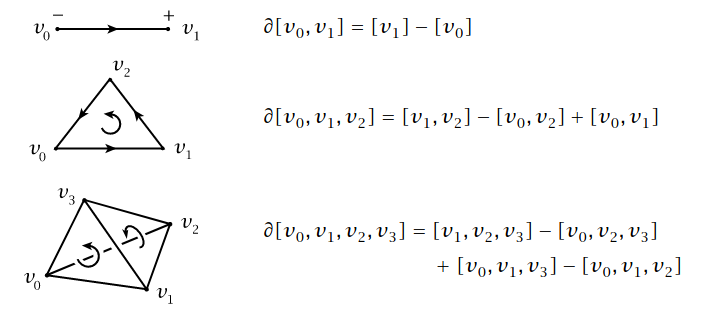
\includegraphics[width = 12cm, height = 6cm]{sections/1/boundary}

    \begin{thm}
        $\del^2 = 0$.
    \end{thm}
    \begin{proof}
        Let $\del_{p+1}([v_0,\dots,v_{p+1}]) = \sum_{i=0}^{p+1} (-1)^i[v_0,\dots,\hat{v_i},\dots,v_{p+1}]$ then 
        \[\del_p(\del_{p+1}([v_0,\dots,v_{p+1}])) =\sum_{j=0, j \neq i}^{p+1} \sum_{i=0}^{p+1} (-1)^{i+j}[v_0,\dots,\hat{v_i},\dots,\hat{v_j},\dots,v_{p+1}] = 0.\]        
    \end{proof}

    \begin{defn}
        We define the \ii{p-homology group} to be $H_p := \frac{im\del_{p+1}}{ker\del_p}$, where $im\del_{p+1}$ is the group of simplicial p-cycles and
        $ker\del_p$ is the group of simplicial p-boundaries.
    \end{defn}

    The homology group is therefore the space of cycles that are not boundaries.

\end{document}
